\section{Background}
\label{sec:background}
In order to formalize the approach of this research, some background information must be supplied. Boolean Satisfiability (SAT) solvers attempt to determine if there exists a total truth assignment to a given propositional formula, that evaluates to TRUE. Generally, a propositional formula is any combination of the disjunction and conjunction of literals (as an example, $a$ and $\neg a$ are literals). For a given unsatisfiable problem, solvers try to generate a proof of unsatisfiability; this is generally more useful than a proof of satisfiability. Such a proof is dependent on identifying a subset of clauses that make the problem unsatisfiable (UNSAT). 

SAT solvers in model checking work over a constraint system to determine satisfiability. A \textit{constraint system} $C$ is an ordered set of $n$ abstract constraints $\{C_1, C_2, ..., C_n\}$ over a set of variables. The constraint $C_i$ restricts the allowed assignments of these variables in some way~\cite{liffiton2016fast}. Given a constraint system, we require some method of determining, for any subset $S \subseteq C$, whether $S$ is \textit{satisfiable} (SAT) or \textit{unsatisfiable} (UNSAT). When a subset $S$ is SAT, this means that there exists an assignment allowed by all $C_i \in S$; when no such assignment exists, $S$ is considered UNSAT. 

The \aivcalg algorithm adapts the MARCO scheme~\cite{liffiton2016fast} which generates all MUSs and applies the idea to sequential model checking~\cite{Ghassabani2017EfficientGO}. Thus, MIVCs are MUSs for inductive systems. \danielle{<-- wording?}

Such a constraint system can encode our example. Consider the first layer of analysis (top level of the system): $C = \{g_p, g_t, g_r, \neg P\}$. This constraint system describes the supporting guarantees at the lower level and the constrained safety property at the top level. The reason for the constraint on $P$ is due to the formulation of the constraint system by the model checker we use, JKind. JKind attempts to look at the unsatisfiability of the problem in order to produce proof results. \danielle{I don't like this description - it can be better. Look over these sentences.}

Given a constraint system $C$, there are certain subsets of $C$ that are of interest in terms of satisfiability. Definitions 2-4 are taken from research by Liffiton et al.,~\cite{liffiton2016fast}. 

\begin{definition} : A Minimal Unsatisfiable Subset (MUS) $M$ of a constraint system $C$ is a subset $M \subseteq C$ such that $M$ is unsatisfiable and $\forall c \in M$ : $M \setminus \{c\}$ is satisfiable. 
\end{definition}
\noindent
An MUS can be intuitively understood as the minimal explanation of the constraint systems infeasability. 

Returning to our running example, this can be illustrated by the following. Given the constraint system $C = \{g_p, g_t, g_r, \neg P\}$, one minimal explanation of the infeasability of this system is the set $\{g_p, g_t, g_r,\}$. If all three guarantees can be violated, then there exists an assignment for all elements such that the system is satisfiable. Given that $P$ is an ``OR" statement of all three guarantees, in order to satisfy $\neg P$, all three guarantees must be violated. Due to the level of the architecture under analysis, there are no faults in the system, but instead only guarantees that may be violated. This is always the case with logical subsystems in a compositional approach. 

\begin{definition} : A Minimal Correction Set (MCS) $M$ of a constraint system $C$ is a subset $M\subseteq C$ such that $C \setminus M$ is satisfiable and $\forall S \subset M$ : $C \setminus S$ is unsatisfiable. 
\end{definition}
\noindent
A MCS can be seen to ``correct'' the infeasability of the constraint system by the removal from $C$ the constraints found in an MCS.

Returning to the PWR example, we can see that if all three guarantees hold, then the safety property $P$ will also hold, i.e., the nominal model is verified. But the constraint system is in terms of $\neg P$ which clearly gives an unsatisfiable constraint system. In this case, we may ask: what will correct this unsatisfiability? These are the MCSs for this constraint system: $MCS_1 = \{g_t\}$, $MCS_2 = \{g_p\}$, $MCS_3 = \{g_r\}$. 

A duality exists between the MUSs of a constraint system and the MCSs as established by Reiter \cite{reiter1987theory}. This duality is defined in terms of \textit{Minimal Hitting Sets} (\textit{MHS}). A hitting set of a collection of sets $A$ is a set $H$ such that every set in $A$ is ``hit'' by $H$; $H$ contains at least one element from every set in $A$. Every MUS of a constraint system is a minimal hitting set of the system's MCSs, and likewise every MCS is a minimal hitting set of the system's MUSs~\cite{liffiton2016fast, reiter1987theory, de1987diagnosing}.

For the PWR top level constraint system, it can be seen that each of the MCSs intersected with the MUS is nonempty. 

Since we are interested in sets of active faults that cause violation of the safety property, we turn our attention to Minimal Cut Sets. 
\begin{definition}
A \textit{Minimal Cut Set} (MinCutSet) is a minimal collection of faults that lead to the violation of the safety property. Furthermore, any subset of a MinCutSet will not cause this property violation. 
\end{definition}
\noindent
We define a minimal cut set consistently with much of the research in this field~\cite{fta:survey,historyFTA}.

\subsection{Inductive Validity Cores}
Given a safety property, a model checker can be invoked in order to construct a proof of the property.  It is often useful to extract traceability information related to the proof, in
other words, which portions of the model were necessary to construct the proof.  Minimal Inductive Validity Cores (MIVCs) describe the minimal
model elements necessary for the inductive proof of a safety property for a sequential system~\cite{GhassabaniGW16}.  MIVCs can be considered a generalization of UNSAT cores for sequential systems.  Further work extended the MIVC algorithms to produce all mimimal sets of MIVC elements (\aivcalg)~\cite{Ghassabani2017EfficientGO,bendik2018online}.  These algorithms are incorporated into the JKind model checker~\cite{2017arXiv171201222G} which is given a model in the dataflow programming language Lustre~\cite{Halbwachs91:IEEE} 

The \aivcalg algorithm collects all minimal unsatisfiable subsets of a given transition system in terms of the \textit{negation} of the top level property~\cite{Ghassabani2017EfficientGO,bendik2018online}. Assuming that the nominal model proves (no faults are active), it is not surprising that the model elements (guarantees and assumptions of components) and the negation of the safety property is UNSAT. The MUSs are the minimal explanation of the infeasibility of this constraint system; equivalently, these are the minimal sets of model elements necessary for proof of the safety property.

\subsection{High Level Overview of the Main Idea}

We utilize the \aivcalg algorithm by providing not only component contracts as model elements, but also faults constrained to \textit{false}, i.e., the faults are inactive. We first check that the property is true of the system when no faults occur; if not, then the system must be repaired until the property is true before starting this analysis.  With this assumption, the resulting the resulting MIVCs (MUSs) will contain the required contracts and constrained faults necessary to prove the safety property. A high level summary of the steps of this transformation are shown in Figure~\ref{fig:trans}. 

\begin{figure*}[h!]
	%\vspace{-0.1in}
	\begin{center}
		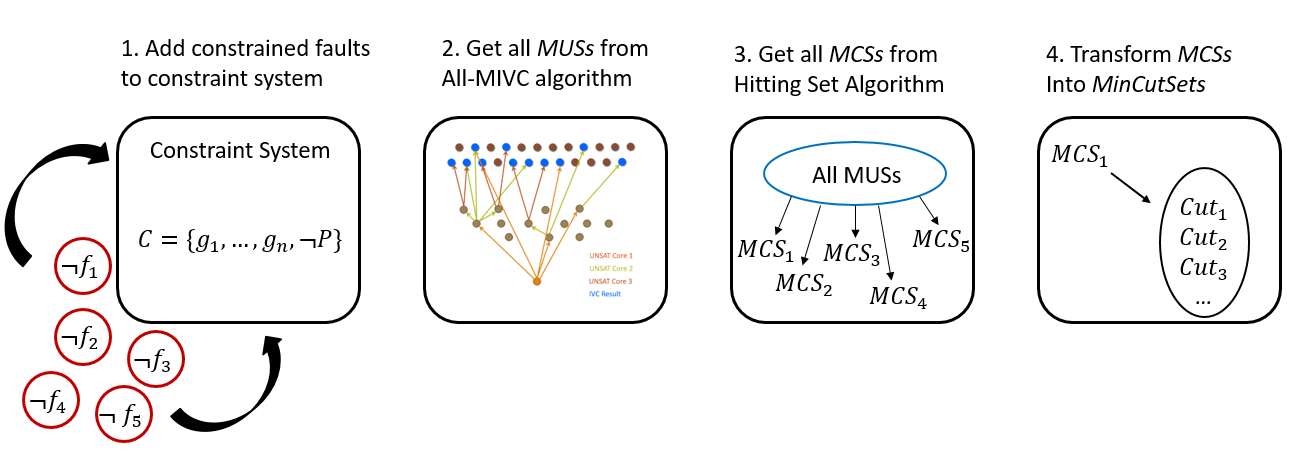
\includegraphics[width=0.6\textwidth]{images/highLevelIdea.PNG}
	\end{center}
	\caption{Steps of the Transformation Process}
	\label{fig:trans}
\end{figure*}

Returning to the PWR example, we focus now on a lower layer of analysis -- proving the guarantee at the temperature subsystem level. The constraint system will now consist of constrained faults of the sensors and the negation of the property of interest $g_t$: $C = \{\neg f_{t1}, \neg f_{t2}, \neg f_{t3}, \neg g_t\}$. 

The MIVCs (or MUSs) of this sytem correspond to all pairs of faults constrained to faults due to the majority voting mechanism. Simply put, if any two faults \emph{occur}, then the negation of $g_t$ is satisfiable. 

Because of the duality between MUSs and MCSs, all MCSs can be obtained by finding the hitting sets of all MUSs. The MCS can be seen to correct the infeasibility of the constraint system and provides the minimal such correction. By removing the constraints from $C$ that are found in any MCS, $C$ becomes satisfiable. In terms of the constraint system that includes fault activation literals, by \textit{activating} the faults in the MCS and \textit{violating} the contracts in the MCS, we can demonstrate the \textit{negation} of the property $P$. 

To illustrate, notice that in the PWR example, all MIVCs are given as: 
$$\boxed{
	\begin{aligned}
		MIVC_1(g_t) = \{\neg f_{t1}, \neg f_{t2}\} \\
		MIVC_2(g_t) = \{\neg f_{t1}, \neg f_{t3}\} \\
		MIVC_3(g_t) = \{\neg f_{t2}, \neg f_{t3}\}
	\end{aligned}
}$$

The hitting sets of all MIVCs are: 
 $$\boxed{
	\begin{aligned}
		MCS_1 = \{\neg f_{t1}, \neg f_{t2}\} \\
		MCS_2 = \{\neg f_{t1}, \neg f_{t3}\} \\
		MCS_3 = \{\neg f_{t2}, \neg f_{t3}\}
	\end{aligned}
}$$

By removing the constraints from the elements in each MCS, we have the ``correction" to the infeasible constraint system; an assignment exists such that $\neg g_t$ is satisfiable. These are the minimal cut sets for $g_t$. 

In summary, if the contracts in the MCS are replaced with the faults that cause its violation, the MCS can be transformed into a MinCutSet. 

%\textbf{Background Information on Toolsuite}
\danielle{My suggestion is to place this at the front of the implementation section. It just seems like it is taking longer to get to the interesting part of the paper by having it here.}

The algorithms in this paper are implemented in the Safety Annex for the Architecture Analysis and Design Language (AADL) and require the Assume-Guarantee Reasoning Environment (AGREE)~\cite{NFM2012:CoGaMiWhLaLu} to annotate the AADL model in order to perform verification using the back-end model checker \jkind~\cite{2017arXiv171201222G}. 

\textbf{Architecture Analysis and Design Language}
We are using the Architectural Analysis and Design Language (AADL) to construct system architecture models of performance-critical, embedded, real-time systems~\cite{AADL_Standard,FeilerModelBasedEngineering2012}. %An AADL model describes a system in terms of a hierarchy of components and their interconnections, where each component can either represent a logical entity (e.g., application software functions, data) or a physical entity (e.g., buses, processors). 
Language annexes to AADL provide a richer set of modeling elements for various system design and analysis needs, and the language definition is sufficiently rigorous to support formal analysis tools that allow for early phase error/fault detection. 

\textbf{Compositional Analysis} 
One way to structure compositional verification is hierarchically: layers of the system architecture are analyzed independently and their composition demonstrates a system property of interest. Compositional verification partitions the formal analysis of a system architecture into verification tasks that correspond into the decomposition of the architecture~\cite{clarke1989compositional}.  A proof consists of demonstrating that the system property is provable given the contracts of its direct subcomponents and the system assumptions~\cite{cofer2012compositional,clarke1989compositional}. When compared to monolithic analysis (i.e., analysis of the flattened model composed of all components), the compositional approach allows the analysis to scale to much larger systems~\cite{NFM2012:CoGaMiWhLaLu,heckel1998compositional,cofer2012compositional}.

\textbf{Assume Guarantee Reasoning Environment}
The Assume Guarantee Reasoning Environment (AGREE) is a tool for formal analysis of behaviors in AADL models and supports compositional verification~\cite{NFM2012:CoGaMiWhLaLu}.  It is implemented as an AADL annex and is used to annotate AADL components with formal behavioral contracts. Each component's contracts includes assumptions and guarantees about the component's inputs and outputs respectively. AGREE translates an AADL model and the behavioral contracts into Lustre~\cite{Halbwachs91:IEEE} and then queries the \jkind model checker to conduct the back-end analysis~\cite{2017arXiv171201222G}. 

\textbf{JKind}
JKind is an open-source industrial infinite-state inductive model checker for safety properties~\cite{2017arXiv171201222G}. Models and properties in JKind are specified in Lustre~\cite{Halbwachs91:IEEE}, a synchronous dataflow language, using the theories of linear real and integer arithmetic. JKind uses SMT-solvers to prove and falsify multiple properties in parallel.

\textbf{Safety Annex for AADL}
The Safety Annex for AADL provides the ability to reason about faults and faulty component behaviors in AADL models~\cite{Stewart17:IMBSA,stewart2020safety}. In the Safety Annex approach, AGREE is used to define the nominal behavior of system components, faults are introduced into the nominal model, and JKind is used to analyze the behavior of the system in the presence of faults. Faults describe deviations from the nominal behavior and are attached to the outputs of components in the system.%The Safety Annex supports behavioral specification of faults and their implicit propagation through behavioral relationships in the model as well as explicit propagation through dependencies. 


